\documentclass[language=german,style=solution]{smo}

\usepackage{tikz}

\title{SMO - Vorrunde 2017 - Lösungen}

\begin{document}

\begin{enumerate}

\item[\textbf{G1)}] 
Sei $ABC$ ein Dreieck mit $AB \neq AC$ und Umkreis $k$. Die Tangente an $k$ durch $A$ schneide $BC$ in $P$. Die Winkelhalbierende von $\angle APB$ schneide $AB$ in $D$ und $AC$ in $E$. Zeige, dass das Dreieck $ADE$ gleichschenklig ist.

\textbf{1. Lösung}
Sei $\alpha := \angle BAC$ und $\beta := \angle CAB$. Mit dem Tangentenwinkelsatz folgt $\angle CAP = \beta$. Wir benutzen nun die Innenwinkelsumme im Dreieck $ABP$ und erhalten $\angle APB = 180^\circ- \alpha - 2 \beta$. Mit der Winkelhalbierenden folgt $\angle APD = 90^\circ - \beta - \frac{1}{2}\alpha$. Die Innenwinkelsumme im Dreieck $ADP$ ergibt $\angle PDA = 90^\circ - \frac{1}{2}\alpha$. Wenn wir nun noch im Dreieck $ADE$ den letzten Winkel $\angle AED = 90^\circ - \frac{1}{2}\alpha$ ausrechnen, sehen wir dass das Dreieck gleichschenklig ist.

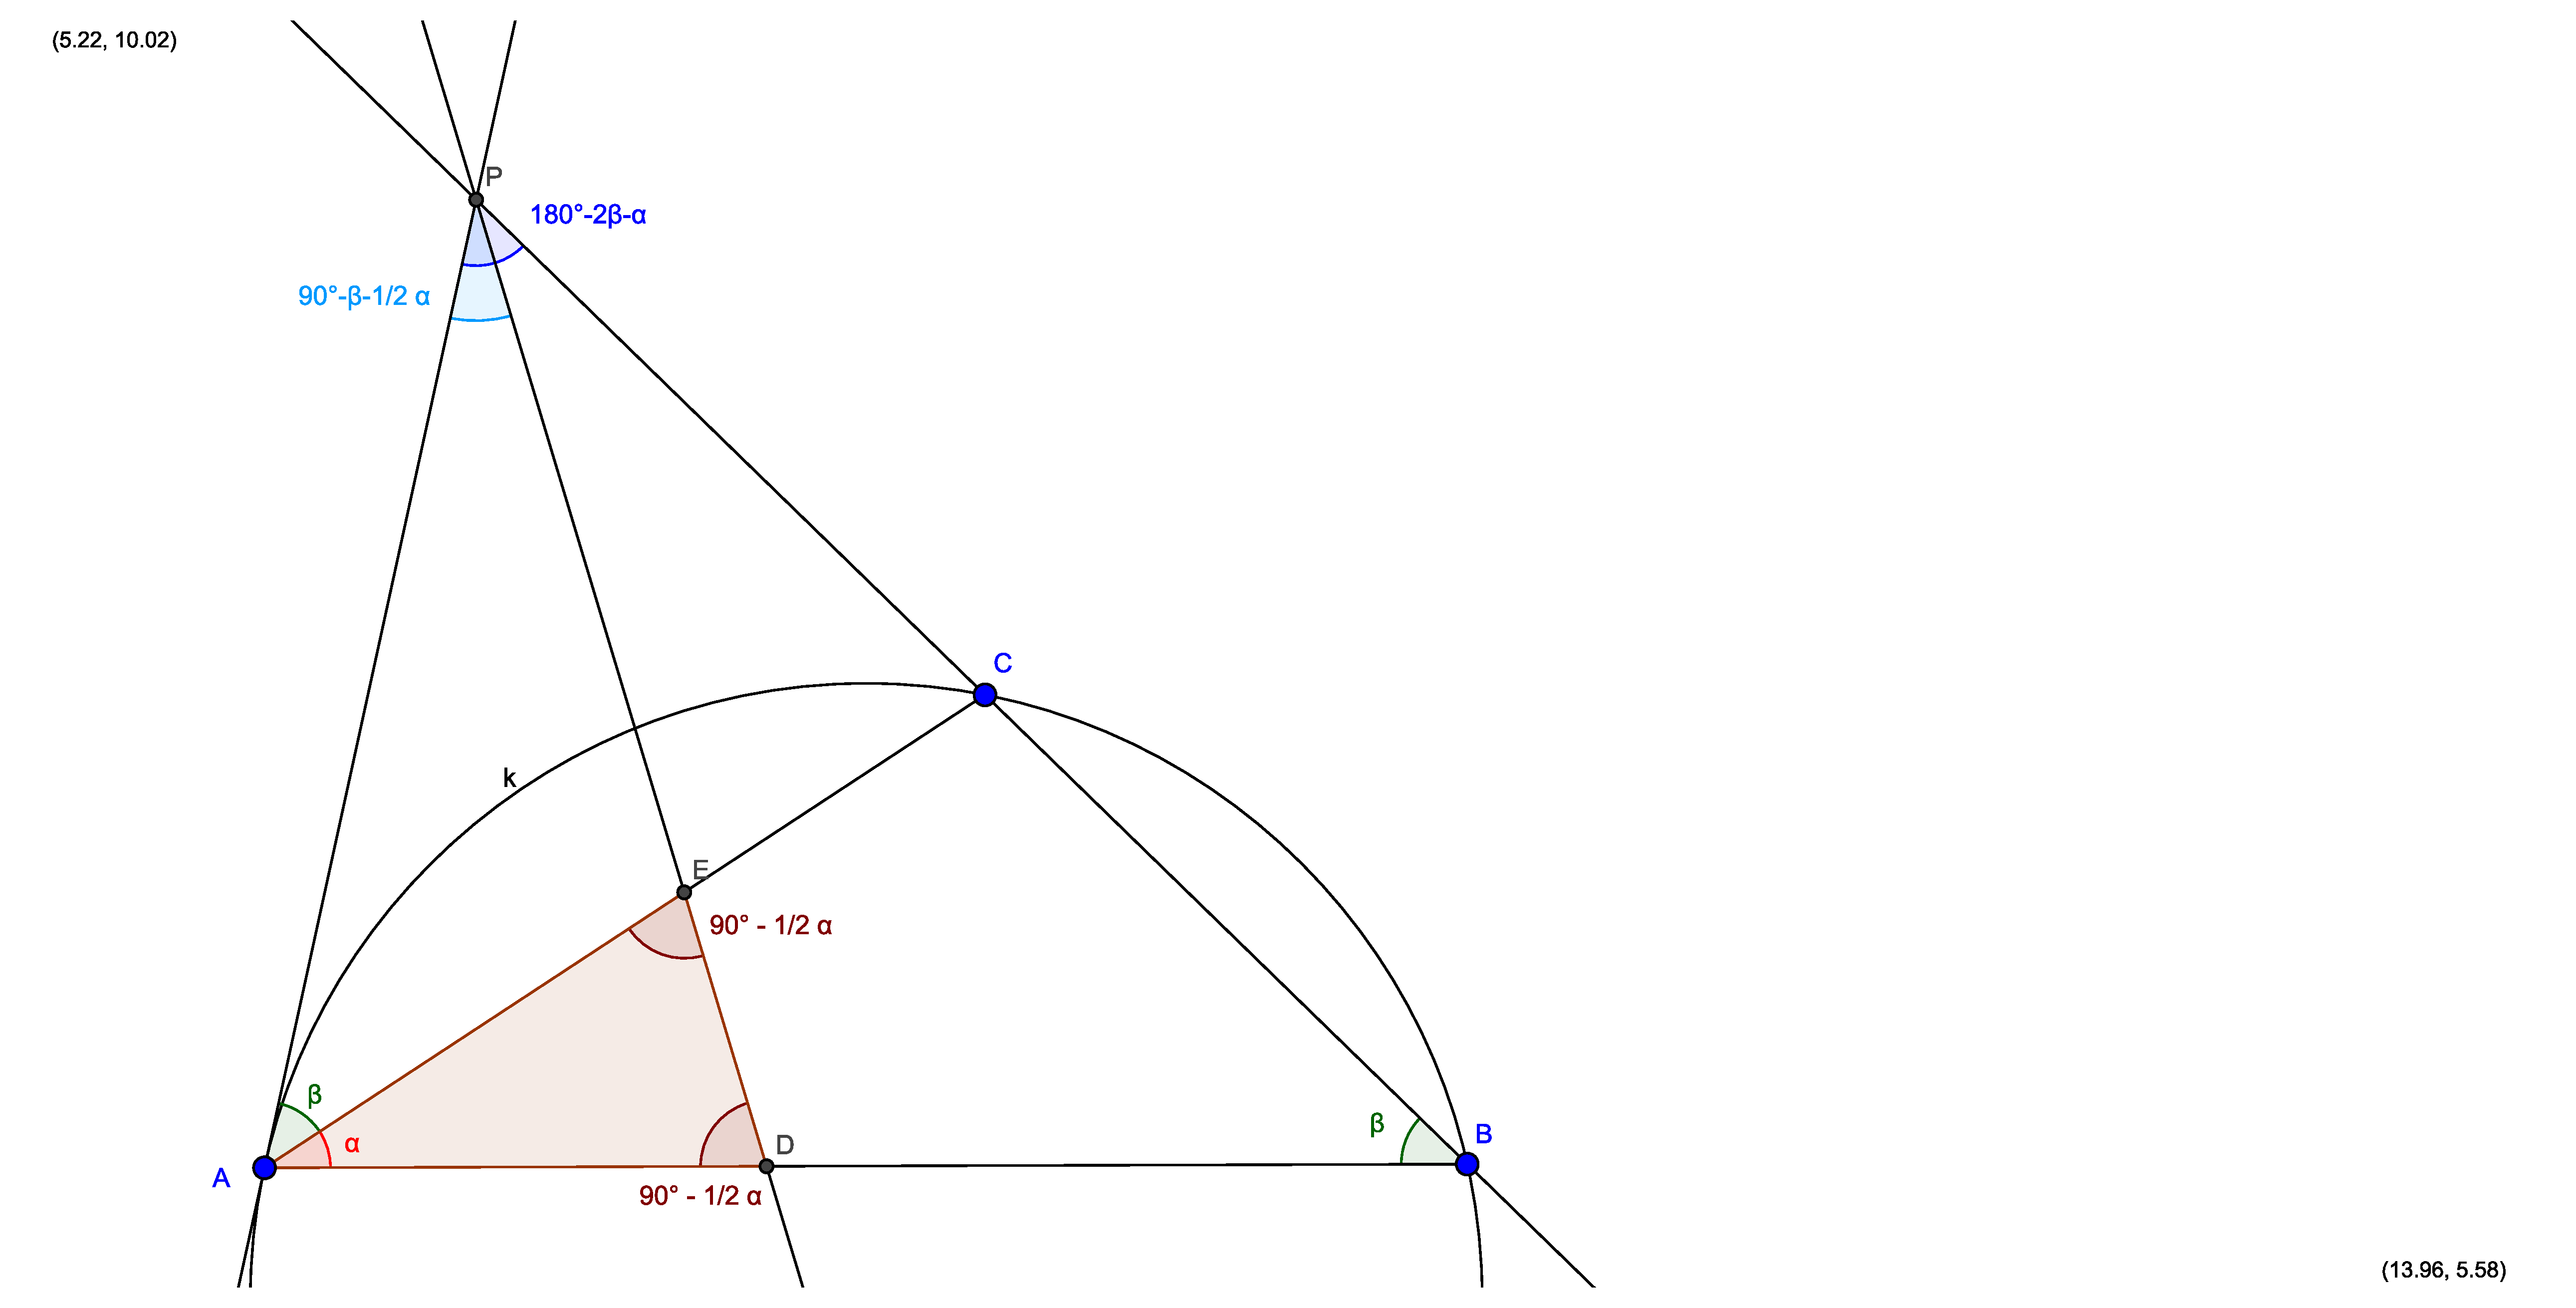
\includegraphics[width=1.5\textwidth,clip=100]{G1.pdf}

\textbf{Marking Scheme}
\begin{itemize}
\item +2 Punkte: $\angle ABC = \angle CAP$ (mit Begründung)
\item +1 Punkt: $\angle APB$ ausgerechnet abhängig von den Winkeln $\alpha$ und $\beta$.
\item +1 Punkt: $\angle APD$ ausgerechnet abhängig von den Winkeln $\alpha$ und $\beta$.
\item +1 Punkt: $\angle PDA$ ausgerechnet abhängig von den Winkeln $\alpha$ und $\beta$.
\end{itemize}

\newpage

\item[\textbf{G2)}] 
Sei $ABC$ ein rechtwinkliges Dreieck mit Hypotenuse $AB$. Ein Kreis um $C$ schneide die Strecke $AB$ zweimal in den Punkten $P$ und $Q$, wobei $P$ zwischen $A$ und $Q$ liegt. Sei $R$ der Punkt auf der Strecke $BC$ mit $\angle RAC=\frac{1}{2}\angle PCQ$ und sei $S$ der Punkt auf der Strecke $AC$ mit $\angle CBS=\frac{1}{2}\angle PCQ$. Weiter sei $T$ der Schnittpunkt der Strecken $CP$ und $AR$, und $U$ der Schnittpunkt der Strecken $CQ$ und $BS$.
Zeige, dass $RSTU$ ein Sehnenviereck ist.

\textbf{Lösung:}

Es gilt:
\[
\angle RAS = \angle RAC = \frac{1}{2}  \angle PCQ = \angle CBS = \angle RBS
\]
Mit der Umkehrung des Peripheriewinkelsatzes folgt, dass $RSAB$ ein Sehnenviereck ist.\\

Da $P$ und $Q$ auf einem Kreis mit Mittelpunkt $C$ liegen, ist das Dreieck $CPQ$ gleichschenklig. Man erhält:
\[
\angle PQC = \frac{1}{2} (180^{\circ} - \angle PCQ) = 90^{\circ} - \frac{1}{2} \angle PCQ = 90^{\circ} - \angle RAC
\]
Aus der Innenwinkelsumme im Dreieck $ARC$ und dem rechten Winkel in $C$ folgt:
\[
\angle ARC = 90^{\circ} - \angle RAC
\]
Somit gilt:
\[
\angle AQC = \angle PQC = \angle ARC
\]
Woraus folgt, dass $AQRC$ ein Sehnenviereck ist.

Mit den beiden Sehnenvierecken $RSAB$ und $AQRC$ erhält man:
\[
\angle RCQ = \angle RAQ = \angle RAB = \angle RSB = \angle RSU
\]
Somit ist $RCSU$ ein Sehnenviereck.\\

Analog findet man das Sehnenviereck $RCST$.\\
Das heisst, dass $U$ und $T$ beide auf dem Umkreis vom Dreieck $RCS$ liegen. Daher ist $RCSTU$ ein Sehnenfünfeck und $RSTU$ ein Sehnenviereck.\\

\textbf{Marking Scheme:}
\begin{itemize}
\item +1: $RSAB$ Sehnenviereck
\item +1: $AQRC$ Sehnenviereck oder analog
\item +2: $RCSU$ Sehnenviereck oder analog
\item +1: analoges Sehnenviereck zu $RCSU$ zusätzlich.
\item fertig
\end{itemize}

\newpage %%%%%%%%%%%%%%%%%

\item[\textbf{K1)}] 
Quel est le nombre maximal de Skew-Tetrominos que l'on peut placer sur un rectangle $8 \times 9$ sans recouvrement?

\textit{Remarque: Les tetrominos peuvent être tournés et réfléchis.}

\textbf{Solution:}
Le nombre maximal de Skew-Tetrominos est $16$.
	
Montrons déjà qu'on peut en placer $16$. On sépare le rectangle en $4$ plus petits rectangles de $2$ lignes et $9$ colonnes. Sur chacun de ces petits rectangles on peut placer $4$ Skew-Tetrominos (en les mettant tous dans l'orientation sur la feuille d'examen), donc on arrive à en placer $16$ sur le rectangle entier.
	
Montrons maintenant qu'on ne peut pas en placer plus que $16$.
	
\textbf{Première solution:} On colorie toutes les colonnes impaires en noir et toutes les colonnes paires en blanc. On remarque alors d'une part que chaque Skew-Tetromino doit recouvrir deux cases blanches et deux cases noires, et d'autre part qu'il y a $40$ cases noires et $32$ cases blanches. Il y a donc au moins $8$ cases noires qui ne seront pas recouvertes par un Tetromino, ce qui signifie que les Tetrominos recouvrent au maximum $64$ cases et donc on ne peut pas en placer plus que $16 = 64/4$.
	
\textbf{Deuxième solution:} On colorie en noir toutes les cases se trouvant dans une colonne paire et dans une ligne paire, et en blanc toutes les autres. On remarque alors d'une part qu'il y a 16 cases noires, et d'autre part que chaque Tetromino doit recouvrir exactement une case noire, donc on peut placer au maximum $16$ Tetrominos.

\textbf{Marking Scheme}
	\begin{itemize}
		\item \textbf{Construction:}\\
			Déduire par une construction que l'on peut placer $16$ Tetrominos: 2 Pts.
		
		\textbf{Première solution:}
		\item Trouver une coloration semblable et constater que chaque Tetromino recouvre deux cases noires et deux cases blanches: 1 Pt.
		\item Trouver une coloration semblable et remarquer qu'il y a $40$ cases noires et $32$ cases blanches: 1 Pt.
%		\item En déduire qu'il doit rester au moins $8$ cases vides: +2 Pts.
		\item En déduire que l'on ne peut pas placer plus de $16$ Tetrominos: +3 Pts.
		
		\textbf{Deuxième solution:}
		\item Trouver une coloration semblable (peut-être avec fausse shift) et remarquer que chaque Tetromino recouvre exactement une case coloriée: 1 Pt.
		\item Trouver une coloration semblable et remarquer qu'il y a $16$ cases coloriées: 1 Pt.
		\item En déduire que l'on ne peut pas placer plus de $16$ Tetrominos: +3 Pt.
	\end{itemize}
On ne peut pas obtenir des points partiels des deux solutions. Si les deux sont essayées, il faut uniquement donner les points d'après celle qui permet d'attribuer le plus grand nombre de points.

\newpage %%%%%%%%%%%%%%%

\item[\textbf{K2)}] 

Seien $m, n\geq 2$ natürliche Zahlen. Wir haben vier Farben und wollen jedes Feld eines $m\times n$ Rechtecks mit einer davon einfärben, sodass in jedem $2 \times 2$ Quadrat alle vier Farben vorkommen. Wie viele verschiedene Möglichkeiten gibt es dafür?

\textit{Bemerkung: Wir zählen zwei Möglichkeiten als verschieden, wenn es mindestens ein Feld gibt, das unterschiedliche Farben erhalten hat.}

\textbf{Lösung:}
Seien zuerst $m,n>2$. Wir ersetzen die Farben der Einfachheit halber durch Zahlen und betrachten drei benachbarte Felder einer Zeile, die alle unterschiedlich gefärbt wurden (ObdA mit 1, 2 und 3). Es folgt der Reihe nach:

$\begin{array}{c|c|c|c|c}
   &  &  &  & \\
  \hline
   &  &  &  & \\
  \hline
   &  &  &  & \\
  \hline
   &1 &2 &3 & \\
  \hline
   &  &  &  & \\
  \hline
   &  &  &  & \\
  \hline
   &  &  &  & \\
\end{array}
\qquad
\begin{array}{c|c|c|c|c}
   &  &  &  & \\
  \hline
   &  &  &  & \\
  \hline
   &  &4 &  & \\
  \hline
   &1 &2 &3 & \\
  \hline
   &  &4 &  & \\
  \hline
   &  &  &  & \\
  \hline
   &  &  &  & \\
\end{array}
\qquad
\begin{array}{c|c|c|c|c}
   &  &  &  & \\
  \hline
   &  &  &  & \\
  \hline
   &3 &4 &1 & \\
  \hline
   &1 &2 &3 & \\
  \hline
   &3 &4 &1 & \\
  \hline
   &  &  &  & \\
  \hline
   &  &  &  & \\
\end{array}
\qquad
\begin{array}{c|c|c|c|c}
 & \vdots & \vdots & \vdots & \\
  \hline
   & 1 & 2 & 3 & \\
  \hline
   & 3 & 4 & 1 & \\
  \hline
   & 1 & 2 & 3 & \\
  \hline
   & 3 & 4 & 1 & \\
  \hline
   & 1 & 2 & 3 & \\
  \hline
 & \vdots & \vdots & \vdots & \\ 
\end{array}$

\bigskip

Also sind die gesamten Spalten, welche die drei 'Startfelder' beinhalten, mit nur je zwei Farben alternierend gefärbt. Insbesondere ist jede Zeile mit mindestens 3 verschiedenen Farben gefärbt.\\
Angenommen, es gäbe gleichzeitig drei benachbarte Felder einer Spalte, die alle unterschiedlich gefärbt wurden:
Dann gäbe es auch drei benachbarte Zeilen, die ebenfalls nur mit je zwei Farben gefärbt sind, Widerspruch!
Folglich bestehen die Zeilen oder die Spalten aus nur je zwei Farben (die sich immer abwechseln müssen). Dies stimmt offensichtlich auch für $m=2$ und $n=2$, also immer.

Wir berechnen nun die Anzahl Möglichkeiten mithilfe dieser Eigenschaft.
Wenn die $m$ Spalten aus nur je zwei Farben bestehen, dann haben wir $6$ Möglichkeiten, die beiden Farben für die erste, dritte, fünfte etc. Spalte zu wählen. Die Farben für die restlichen Spalten sind dann eindeutig bestimmt. Wir können nun aber für alle m Spalten noch auswählen, mit welcher der beiden möglichen Farben wir beginnen ($2^m$ Möglichkeiten), insgesamt also $6*2^m$ Möglichkeiten. Analog liefert der Fall, dass die Zeilen aus nur je zwei Farben bestehen, weitere $6\cdot2^n$ Möglichkeiten. Nun haben wir allerdings die Fälle doppelt gezählt, in denen sowohl die Zeilen als auch die Spalten nur aus je zwei Farben bestehen. Alle diese Färbungen sind bereits eindeutig definiert, wenn wir das obere linke $2\times2$-Quadrat färben. Dafür gibt es $4\cdot3\cdot2$ Möglichkeiten. Insgesamt erhalten wir also $6\cdot2^m+6\cdot2^n-24$ Möglichkeiten.

\textbf{Marking Scheme:}
\begin{itemize}
\item +4: Beweis, dass Zeilten ode rSpalten nur je 2 Farben enthalten
\item +3: fertig machen
\item -1: für kleine Fehler z.B. vergessen, die Schnittmengen abzuziehen
\end{itemize}

\newpage %%%%%%%%%%%%%%%%

\item[\textbf{Z1)}] 

\textbf{1. Lösung:}
\\
Wir substituieren $m = ad$ und $n=bd$ wobei $d = ggT(m,n)$. Somit ist $kgV(m,n) = abd$. Somit erhalten wir
\[
abd - d = \frac{abd^{2}}{5}.
\]
Das ist äquivalent zu
\[
5 = (5-d)ab.
\] 
Da $a$ und $b$ positiv sind, ist $5-d > 0$ und $5-d \mid 5$. Man sieht das $d = 4$ gelten muss. Also muss $ 5 = ab$ gelten. Daraus folgt $a = 1$ und $b = 5$ oder umgekehrt. Somit ist $(m,n)$ gleich $(4,20)$ oder $(20,4)$.
\\
\\
\textbf{2. Lösung:}
\\
\\
Wir benutzen die analoge Substitution wie in der 1. L\"{o}sung und formen die erhaltene Gleichung zu folgendem um:
\[
abd = 5(ab-1).
\]
Wir sehen $a \neq 1$ oder $b \neq 1$ sonst ist die rechte Seite $0$ und die linke Seite nicht. Daraus folgt $a = 5$ und $b = 1$ oder umgekehrt, da $ggT(ab-1,ab) = ggT(ab-1,1) = 1$, und somit $ab = 5$. Daraus folgt $d = ab -1 = 4$. Somit erhalten wir wieder die beiden L\"{o}sungspaare. 
\\
\\
\textbf{Marking Scheme:} 
\begin{itemize}
\item $+2P$ die benutzte Substitution in die Gleichung eingesetzt. 
\item $+3P$ $d=4$ oder $ab=5$.
\item $7P$ vollständige Lösung
\item $-1P$ Vergessen eines Paares
\end{itemize}
\textbf{3. L\"{o}sung:}
\\
\\
Wir substituieren $mn = ggT(m,n)kgV(m,n)$. Somit erhalten wir
\[
kgV(m,n) - ggT(m,n) = \frac{ggT(m,n)kgV(m,n)}{5}.
\]
F\"{u}r $ggT(m,n) \geq 5$ erhalten wir
\[
kgV(m,n) - ggT(m,n) < kgV(m,n) \leq \frac{ggT(m,n)kgV(m,n)}{5}.
\]
Also gilt $ggT(m,n) \leq 4$. Durch durchtesten erhält man die einzige Möglichkeit $ggT(m,n) = 4)$ und $kgV(m,n) = 20$. Dies impliziert, dass die schon bekannten Lösungen die einzigen beiden sind.
\\
\\
\textbf{Marking Scheme:} 
\begin{itemize}
\item $+2P$ Substitution 
\item $+3P$ $ggT(m,n) \leq 4$ 
\item $7P$ vollständige Lösung
\item $-1P$ Vergessen eines Paares
\end{itemize}

\textbf{4. Lösung:}
Forme um zu
\[
5kgV(m,n)-5ggT(m,n) = mn.
\]
Nehme an, dass die Primzahl $p$ erfüllt $p^k\div m$ aber nicht $p^k\div n$. Dann teilt $p^k$ die rechte Seite, den linken Term der linken Seite, also muss $p^k \mid 5ggT(m,n)$ gelten. Der maximale Exponent $l$, so dass $p^l \mid ggT(m,n)$ gilt, ist kleiner gleich $k-1$. Somit gilt $p\mid 5$ beziehungsweise $p = 5$. Falls $l \leq k-2$ müsste $25\mid 5$ gelten. Somit ist $l = k-1$. Somit gilt $m=5n$ oder $m=n$. Analog kann man die Prozedur umgekehrt machen und man erhält die Möglichkeit $n=5m$. Einsetzen liefert die bekannten Paare.
\\
\textbf{Marking Scheme:}
\begin{itemize}
\item $+1P$ $p^k \mid 5ggT(m,n)$, dieser Punkt ist auch möglich falls man einfach eine Primzahl $q$ betrachtet, welche $m$ und nicht $n$ teilt, und dann erhält $q \mid 5ggT(m,n)$.
\item $+1P$ $p=5$ beziehungsweise $q=5$, falls nicht Potenzen betrachtet werden.
\item $+3P$ $n=5m$, $m=5n$ und $m=n$ sind die einzigen Möglichkeiten. Falls nicht Primpotenzen betrachtet werden, hier nur $+2P$ und $4P$ ist die maximale Anzahl an Punkten die ohne Betrachtung von Primpotenzen erreicht werden kann.
\item $7P$ vollständige Lösung
\item $-1P$ Vergessen eines Paares
\end{itemize}

\textbf{Bemerkungen zu den Marking Schemes:}
\begin{itemize}
\item Die Punkte aus verschiedenen L\"{o}sungen sind nicht additiv, d.h. man erh\"{a}lt Punkte nur f\"{u}r den Weg, wo man am Weitesten ist.
\item F\"{u}r Ungereimtheiten in der Argumentation wird individuell das Mass des Punkteabzugs entschieden.
\end{itemize}

\newpage %%%%%%%%%%%%%%%%%%%

\item[\textbf{Z2)}] 
Seien $a$ und $b$ natürliche Zahlen, sodass
\[
\frac{3a^2+b}{3ab+a}
\]
eine ganze Zahl ist. Bestimme alle Werte, die obiger Ausdruck annehmen kann.

\textbf{Lösung:}

$3ab+a=a(3b+1)$ teilt $3a^2+b$, also ist insbesondere $a$ ein Teiler von $3a^2+b$. Nun teilt $a$ ebenfalls $3a^2+b-(3a)a=b$. Somit können wir $b=as$ schreiben. Einsetzen in den Ausdruck liefert $3a^2s+a\div 3a^2+as$ und nach kürzen mit $a$ bekommen wir $3as+1\div 3a+s$. Da $a$ und $s$ natürliche Zahlen sind, ist $3a+s$ positiv. Es muss also gelten, dass $3as+1\leq 3a+s$ ist. Falls $s\geq2$ ist, können wir aber wie folgt abschätzen:
\[
3as+1=2as+as+1\geq 4a+as+1\geq 4a+s+1>3a+s, 
\]
wobei wir bei der ersten Ungleichung $s\geq 2$ und bei der zweiten Ungleichung $a\geq 1$ brauchen. Dies ist ein Widerspruch zu der Bedingung $3as+1\leq 3a+s$, also muss $s<2$ sein. Es folgt $s=1$ und damit $a=b$. Einsetzen von $a=b$ in den gegebenen Ausdruck liefert $\frac{3a^2+a}{3a^2+a}=1$. Somit ist $1$ der einzige Wert, der angenommen werden kann. Dieser Wert wird für alle Paare $(a,a)$ natürlicher Zahlen angenommen.

Statt der Abschätzung kann man ebenfalls die Ungleichung $3as+1\leq 3a+s$ umformen zu $0\geq (3a-1)(s-1)$. Da $3a-1$ für jedes $a$ positiv ist, darf $s-1$ nicht positiv sein. Somit muss $s=1$ gelten. Wir können wie oben fertigmachen.

\textbf{Marking Scheme}
\begin{itemize}
	\item 1 Punkt für $a\div b$.
	\item 1 Punkt für $3as+1\div 3a+s$.
	\item 1 Punkt für $3as+1\leq 3a+s$.
	\item 3 Punkte für $s=1$. \\2 Punkte für obere Schranke an $a$ oder $s$, die kleiner als 5 ist? \\Bei Lösungsweg 2: 1 Punkt davon für Umformung der Ungleichung.
	\item 1/2 Punkt/e für Fertigmachen.
	\item Keine Punkte dafür, dass der Wert 1 angenommen werden kann.
\end{itemize}

\newpage

\end{enumerate}

\end{document}
